\section{Density Matrix and Entropy for Networks}
%as in paper 2023 with the special case in paper 2020
The communicability matrix defined above possesses peculiar properties that make it suitable for use as a density matrix. Moreover, the presence of the Laplacian matrix ensures that it consider not only the topological features of the network but also its dynamics. Taking the exponential communicability matrix as a reference, we can define a density matrix as
\begin{equation}\label{density_matrix}
    \hat \rho(\beta) = \frac{1}{Z} e^{-\beta \hat L} \qquad \text{with} \qquad Z(\beta) = \Tr[e^{-\beta \hat L}],
\end{equation}
where $Z$ is the partition function, which is equal to the Laplacian Estrada index of the network \eqref{EE_L}.
The density matrix $\hat \rho(\beta)$ is a Hermitian and positive definite matrix with trace equal to unity. 
the density matrix $e^{-\beta L}$ is similar to the propagator of the master equation \eqref{random_walk_solution} considering time $t = \beta$.

From this, we can define the network's entropy as the von Neumann entropy
\begin{equation} \label{entropy}
    S(\hat\rho) = -\Tr[\hat \rho \ln \hat \rho].
\end{equation}
The entropy is not negative and equal to zero if and only if the $\hat\rho$ is a pure state. It has a upper bound give by $S \leq \ln(N)$,  \cite{Nielsen_Chuang_2010}.
The entropy satisfies the sub-additivity property \cite{De_Domenico_2016}:
Let $\hat\rho$, $\hat\tau$ and $\hat\sigma$ be density matrices corresponding to the networks $G$, $H$, $I$ respectively. If the networks $H$ and $I$ are subgraphs of the network $G$ such that $G = H + I$.
If the sub-additivity is satisfied we have that $S(\hat\rho) \leq S(\hat\tau) + S(\hat\sigma)$, the equivalence is obtain if the two subgraphs do not have nodes from the same component of $G$. A mathematical proof can be found in appendix \ref{C_sub_additivity}.

Figure \ref{fig:ER-BA-WS} shows the entropy \eqref{entropy} for different types of networks\footnote{The Python scripts can be found on the author's GitHub page at the following link: \url{https://github.com/ShqemzaMatteo/Master_thesis}}: a ring graph, an Erd\H{o}s-Rényi (E-R) random graph, a Barab\'asi-Albert (B-A) scale-free graph, and a Watts-Strogatz (W-S) small-sworld graph.

\begin{figure}[ht!]
    \centering
    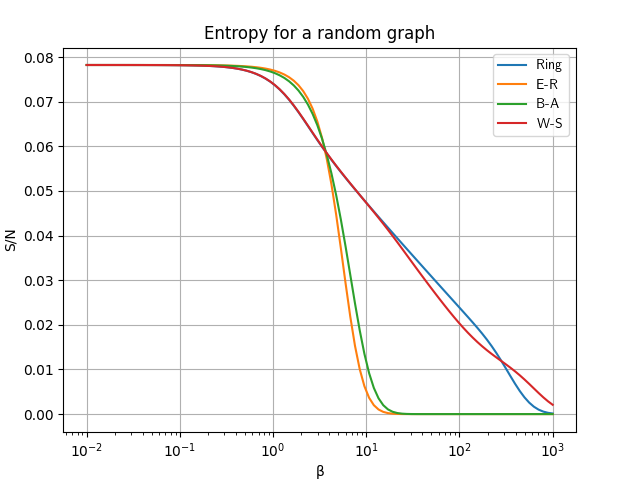
\includegraphics[width=0.80\linewidth]{image/random_graph.png}
    \caption{Plot of the network's entropy per node as a function of $\beta$ for different network types with $50$ nodes: a ring graph (blue), a Erd\H{o}s-Rényi (E-R) random graph with connectivity probability $0.7$ (orange), a Barab\'asi-Albert (B-A) scale-free graph with parameter $m=3$ (green), and a Watts-Strogatz (W-S) small world graph with parameter $K=3$ and rewire probability 0.2 (red). The x-axis is on logarithmic scale. For large $\beta$, the entropy tends to zero for all the networks.}
    \label{fig:ER-BA-WS}
\end{figure}

%Using the density matrix, we can introduce also other thermodynamics quantities like the Helmoltz free energy $F = -\frac{1}{\beta} \ln Z$.

The parameter $\beta$ in the network's entropy suppresses the spread of information along eigenvector with high eigenvalue. In fact, increasing $\beta$, more eigenvalues are suppressed until only the zero eigenvector remains. 
Figure \ref{Fig:eigen_distribution} shows the eigenvalues of the same networks we have studied in figure \ref{fig:ER-BA-WS}. In the ER and BA networks the eigenvalues are clustered around $1$, consequently, their entropy drops rapidly because, when $\beta$ is high enough, their eigenvector are suppressed simultaneously. In contrast, in the ring and WS network the eigenvalues are closer to zero, thus   the suppressed of their eigenvectors is slower.

\begin{figure}[ht!]
    \centering
    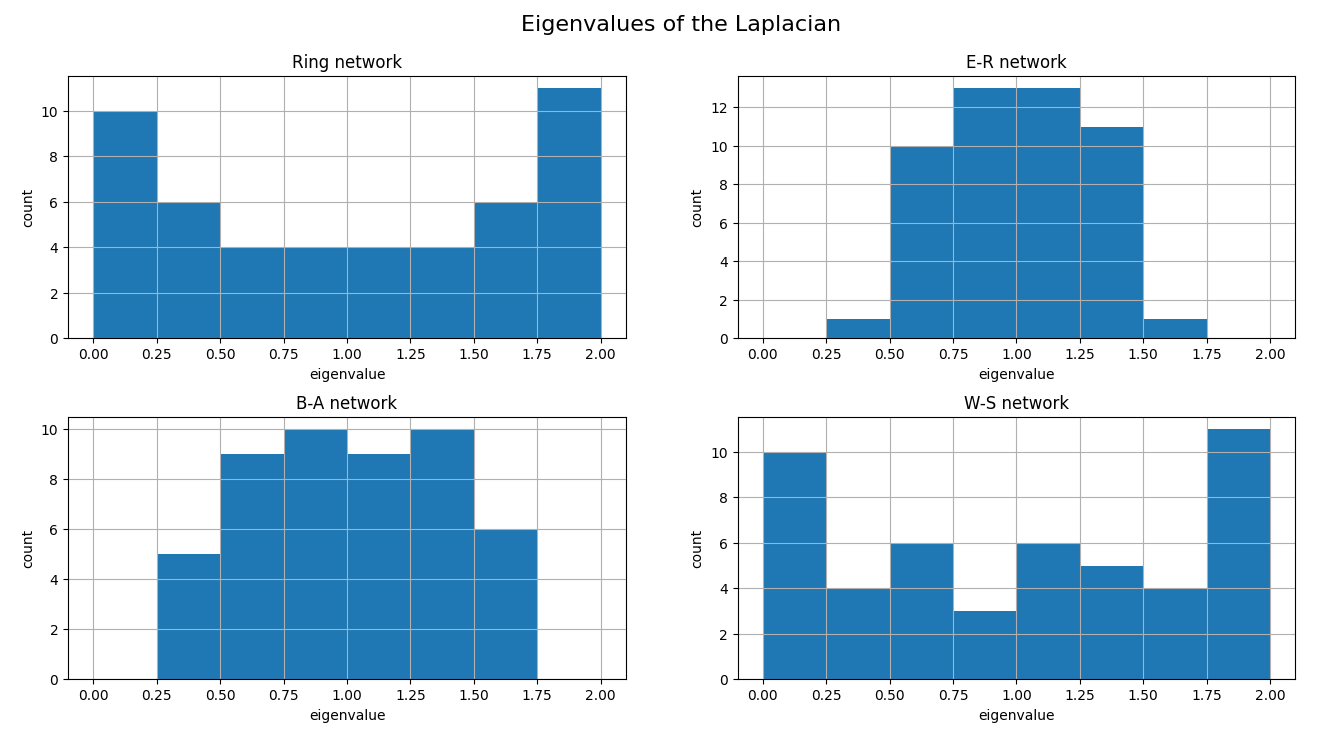
\includegraphics[width=\textwidth]{image/eigenvalue_distribution.png}
    \caption{The figure shows the eigenvalue of the Laplacian matrix for different networks with $50$ nodes: the top left graph is for a ring network, the top right one is for a Erd\H{o}s-Rényi (E-R) random graph with connectivity probability $0.7$, the bottom left one is for a Barab\'asi-Albert (B-A) scale-free graph with parameter $m=3$, the bottom right one shows a Watts-Strogatz (W-S) small world graph with parameter $K=3$ and rewire probability 0.2. In the ring and WS networks the eigenvalues are clustered close to zero and near the value $2$. In contrast, in the ER and BA networks the eigenvalues are clustered around the value $1$.}
    \label{Fig:eigen_distribution}
\end{figure}



A possible interpretation of this density matrix is given by De Domenico \cite{De_Domenico_2020}.
Consider a network $G(N,M)$, represented by the adjacency matrix $A$. In this network, a classic particle performs a random walk. 
The network can be described using the Dirac notation. Let be $\ket{\psi} = \sum_i \rho_i \ket{i}$ the state of the system, where $\ket{i}$ is the canonical vector identifying node $i$ and $\rho_i$ is the probability of finding the particle on top of node $i$. Thus, the scalar product $\braket{i}{\psi} = \rho_i$ is already an observable. The set $\{\ket{i}\}_{i=0}^N$ forms an orthogonal basis, satisfying $\braket{i}{j} = \delta_{ij}$, where $\delta_{ij}$ is the Kronecker delta. 
The evolution of the dynamics is governed by the Laplacian operator $\hat L = L_{ij} \ket{i}\bra{j}$ following the equation
\begin{equation} \label{time_evolution}
    \partial_t \ket{\psi(t)} = - \hat L \ket{\psi(t)},
\end{equation}
with the solution
\begin{equation}
    \ket{\psi(t)} = \hat G(t,0) \ket{\psi(0)}
\end{equation}
where $\hat G(t,0) = e^{-t\hat L}$ is the propagator and $\ket{\psi(0)}$ is the initial state. 

If the detailed balance condition \eqref{detail_condition} holds, $\hat L$ is Hermitian. Therefore, the propagator can be diagonalized in the orthogonal basis $\{\ket{v_\lambda}\}_\lambda$ of eigenvectors of the control operator as
\begin{equation}\label{diagonal_propagator}
    \hat G(t,0) = \sum_\lambda e^{-t\lambda} \ket{v_\lambda}\bra{v_\lambda} = \sum_\lambda e^{-t\lambda} \hat \sigma_\lambda,
\end{equation}
where $\hat \sigma_\lambda = \ket{v_\lambda}\bra{v_\lambda}$ is the projector into the left and right eigenvectors with the $\lambda$ eigenvalue. The operators do not depend on time; they are constant throughout the process, only the coefficients change.
The system relaxes to a stationary state $\ket{\psi_0}$ corresponding to the zero eigenvector.

We consider the system in the initial state $\ket{\psi} = \ket{\psi_0} + \ket{\Delta\psi}$, where $\ket{\Delta\psi}$ is a small perturbation relative to the stationary state. The initial perturbation can be decomposed between the different nodes as $\ket{\Delta\psi_0} = \sum_i \Delta_i \ket{i}$.
The time evolution of the initial state becomes
\begin{equation}
    \ket{\psi(t)} = G(t,0) \ket{\psi(0)} = \ket{\psi_0} + G(t,0)\ket{\Delta\psi} = \ket{\psi_0} + \ket{\Delta\psi(t)}
\end{equation}
with $\ket{\Delta\psi(t)} = e^{-t\hat L} \ket{\Delta \psi}$.

Since the stationary component is constant in time, we focus on the evolution of the perturbation $\ket{\Delta\psi_0}$. 
The value of the perturbation on top of node $j$ at time $t$ is
\begin{equation}
    \braket{j}{\Delta\psi(t)} = \bra{j} e^{-t\hat L} \ket{\Delta\psi} =\sum_\lambda \bra{j} e^{-t\lambda} \hat \sigma_\lambda\ket{\Delta\psi} = \sum_i  \sum_\lambda \Delta_i e^{-t\lambda} \bra{j}  \hat \sigma_\lambda \ket{i}.
\end{equation}
We have used equation \eqref{diagonal_propagator} and the definition of the perturbation.
This equation shows that the perturbation can travel through $N$ different streams, one for each projector $\sigma_\lambda$, with stream's size $\Delta_i e^{-t\lambda}$. If $\Delta_i e^{-t\lambda} > 0$ the stream is active; if $\Delta_i e^{-t\lambda} = 0$ it is inactive. Negative stream coefficients imply an inverted flux from $j$ to $i$.
Now, we assume that there is maximal uncertainty in the perturbation, therefore $\Delta_i = \Delta$.
The dynamics can trap part of the perturbation in a specific node. The size of the trapped perturbation can be compute as
\begin{equation}\label{T_equation}
    T = \sum_i  \sum_\lambda \Delta e^{-t\lambda} \bra{i}  \hat \sigma_\lambda \ket{i} = \Delta \Tr [\hat G(t,0)]
\end{equation} 
We can introduce a density matrix defined as
\begin{equation}
    \hat\rho(t) = \frac{1}{Z}\sum_\lambda  e^{-t\lambda} \hat \sigma_\lambda = \frac{1}{Z} e^{-t\hat L},
\end{equation}
where $Z = \Tr[e^{-t\hat L}] $ is the partition function.
Thus, the evolution of the perturbation yields
\begin{equation}
    \braket{j}{\Delta\psi(t)} = \sum_i \Delta Z \bra{j}\hat\rho(t) \ket{i} = \sum_i T\bra{j}\hat\rho(t) \ket{i}.
\end{equation}
The size of the streams is proportional to the trapped field.
The density matrix can be interpreted as the probability that the perturbation will flow through a specific stream $\hat \sigma_l$ at time $t$ in the ensemble of all the possible streams \cite{De_Domenico_2020}. We have recovered the density matrix \eqref{density_matrix} considering the time $t$ as the parameter $\beta$.

The complexity of information streams can be quantified by the von Neumann entropy.
When the information dynamics is described by a single information stream, entropy vanishes: the density matrix is a pure state.
In contrast, as the information dynamics becomes more complex and diverse, the number of information streams increases, resulting in higher entropy: the density matrix becomes a mixed state.

Considering the analogy with the quantum mechanics, in the following chapters we propose an alternative way to obtain the density matrix \eqref{density_matrix} starting from the quantum walk instead of the classical one. The new description, based on open quantum systems, adds new meaning to the network's entropy \eqref{entropy}.

\subsection{Kullback-Leibler and Jensen-Shannon Divergences}
Starting from the concept of entropy, we can introduce the Kullback-Leibler (KL) divergence or relative entropy \cite{K-L_divergence} as
\begin{equation}\label{KL_divergence}
    D_{KL}(\hat \rho || \hat \sigma) = \Tr \left[\hat \rho \ln\left(\frac{\hat\sigma}{\hat\rho}\right)\right].
\end{equation}
It measures how closely the distribution $\hat \sigma$ reproduces an event to real distribution $\hat \rho$. 
The KL divergence is always non negative and it equals zero when $\hat \rho = \hat \sigma$. It is not symmetric and unbounded \cite{J-S_divergence}.

The KL divergence can be used to make comparisons between networks. Moreover, this concept can be applied to the reconstruction of networks starting from real data using the maximum likelihood estimation: it consists of finding the best model that reproduces the experimental data by minimizing the Kullback-Leibler divergence between a chosen network model and the dataset \cite{De_Domenico_2016}. This opens the door to the application of machine learning techniques in network theory.

However the Kullback-Leibler divergence is not symmetric, therefore it cannot be use as a metric. 
But, we can symmetrize introducing the Jensen-Shannon (JS) divergence \cite{J-S_divergence} defined as
\begin{equation}\label{JS_metric}
    \mathcal{D}_{JS}(\hat\rho||\hat\sigma) =  \frac{1}{2}D_{KL}(\hat \rho || \hat \mu) + \frac{1}{2}D_{KL}(\hat \sigma || \hat \mu) = S(\hat\mu)-\frac{1}{2}\left[S(\hat\rho) + S(\hat\sigma)\right],
\end{equation}
where $\hat\mu =\frac{1}{2}(\hat\rho+\hat\sigma)$. 

The JS divergence is a bounded function \cite{J-S_divergence}
\begin{equation}
    0 \geq \mathcal{D}_{JS}(\hat\rho||\hat\sigma) \geq 1.
\end{equation}
The quantity $\left(\mathcal{D}_{JS}\right)^{\frac{1}{2}}$ defines a metric: it is symmetric, positive definite, and it satisfies the triangle inequality \cite{Jensen-Shannon_divergence}. 
%It has been use successfully to measure the distance between the layer of a multilayer network in order to aggregate them and eliminate the redundant layers \cite{multilayer}.

Figure \ref{Fig:JS_divergence} shows the Jensen-Shannon divergence between an Erd\H{o}s-Rényi (E-R) random graph, a Barab\'asi-Albert (B-A) scale-free graph and a Watts-Strogatz (W-S) small-sworld graph \footnote{TThe Python scripts can be found on the author's GitHub page at the following link: \url{https://github.com/ShqemzaMatteo/Master_thesis}}.

\begin{figure}[ht!]
    \centering
    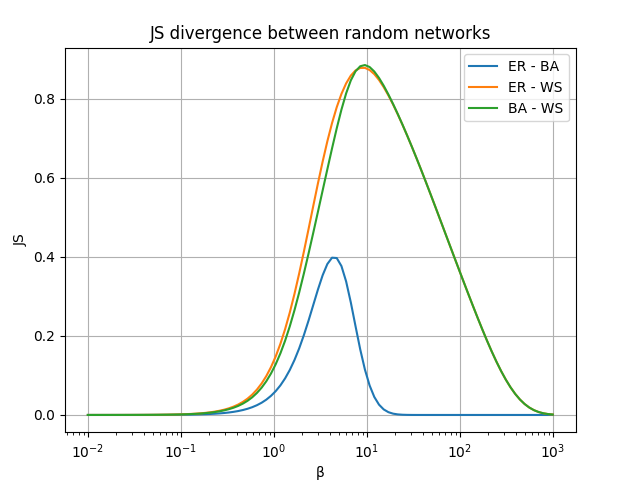
\includegraphics[width=0.80\textwidth]{image/JS_divergence.png}
    \caption{Plot of the KL divergence as a function of $\beta$ between different network types with $50$ nodes: a Erd\H{o}s-Rényi (E-R) random graph with connectivity probability $0.7$ and a Barab\'asi-Albert (B-A) scale-free graph with parameter $m=3$ (blue); a Erd\H{o}s-Rényi (E-R) random graph with connectivity probability $0.7$ and Watts-Strogatz (W-S) small world graph with parameter $K=3$ and rewire probability 0.2 (orange); a Barab\'asi-Albert (B-A) scale-free graph with parameter $m=3$ and a Watts-Strogatz (W-S) small world graph with parameter $K=3$ and rewire probability 0.2 (green). The x-axis is on logarithmic scale. The ER and BA networks are closer in terms of KL divergence compared to the WS network. Notably, the divergence reaches its maximum around $\beta = 10$.}
    \label{Fig:JS_divergence}
\end{figure}
The JS divergence has been use successfully used to measure the distance between the layers of a multiplex network.
In some systems, the elements can interacts through different type of interaction. To models them, we create a set of networks with the same number of nodes but different links, one for each interaction's type. Each network forms a layer in a multiplex. For example, the mobility within a city can be mapped into a multiplex, one layer for each means of transport. Multiplex with many layers are difficult to handle; in order to simplify the model we can use the JS divergence to aggregate the redundant layers \cite{multilayer}.

However, both the KL and JS divergences study only the spectral properties of the system. Thus, they do not distinguish between different networks with same spectrum but different eigenvectors.